\documentclass[]{article}
\usepackage{graphicx}
\usepackage{amsmath,amssymb,amsthm}
\usepackage{empheq}
\usepackage{float}
\usepackage[left=0.85in,top=0.85in,right=0.85in,bottom=0.85in]{geometry} % Document margins

% Title Page
\title{CS 6640 Project 3}
\author{Travis Allen, u1056595}


\begin{document}
	\maketitle
	
	\newpage
	\section{Part 1: FFT's}
	\textbf{Use the built-in FFT functions in python (i.e., numpy) to compute the Fourier transform of some images and show their power spectrum.  You should organize the frequencies so that zero is in the middle of the FFT result/images.  You might need to use a log to see the power clearly.   Show results on several images and comment on what you see in both domains.  Implement a lower pass filter in the Fourier domain and do the inverse FFT to show the effects on several images.}

	\vskip 10pt

	Please see \texttt{problem\_1.py} for how I implemented this. 
	
	\vskip 10pt
	
	\textbf{Images and their FFTs}
	I used the \texttt{numpy.fft.fft2()} function to compute the discrete fast fourier transform of each of my images. Then, I used \texttt{numpy.fft.fftshift()} to ``retile" each image so that the center of each image corresponds to a frequency of zero. The only purpose of this step is to make the results (both intermediate and final) easier to digest. Then, I computed the log of the power spectrum of each image so the results were easier to see. These results are shown below for each image.
		
	%-------------------------------------------------------------------------------------------
	% image 0
	\begin{figure}[H]
		\centering
		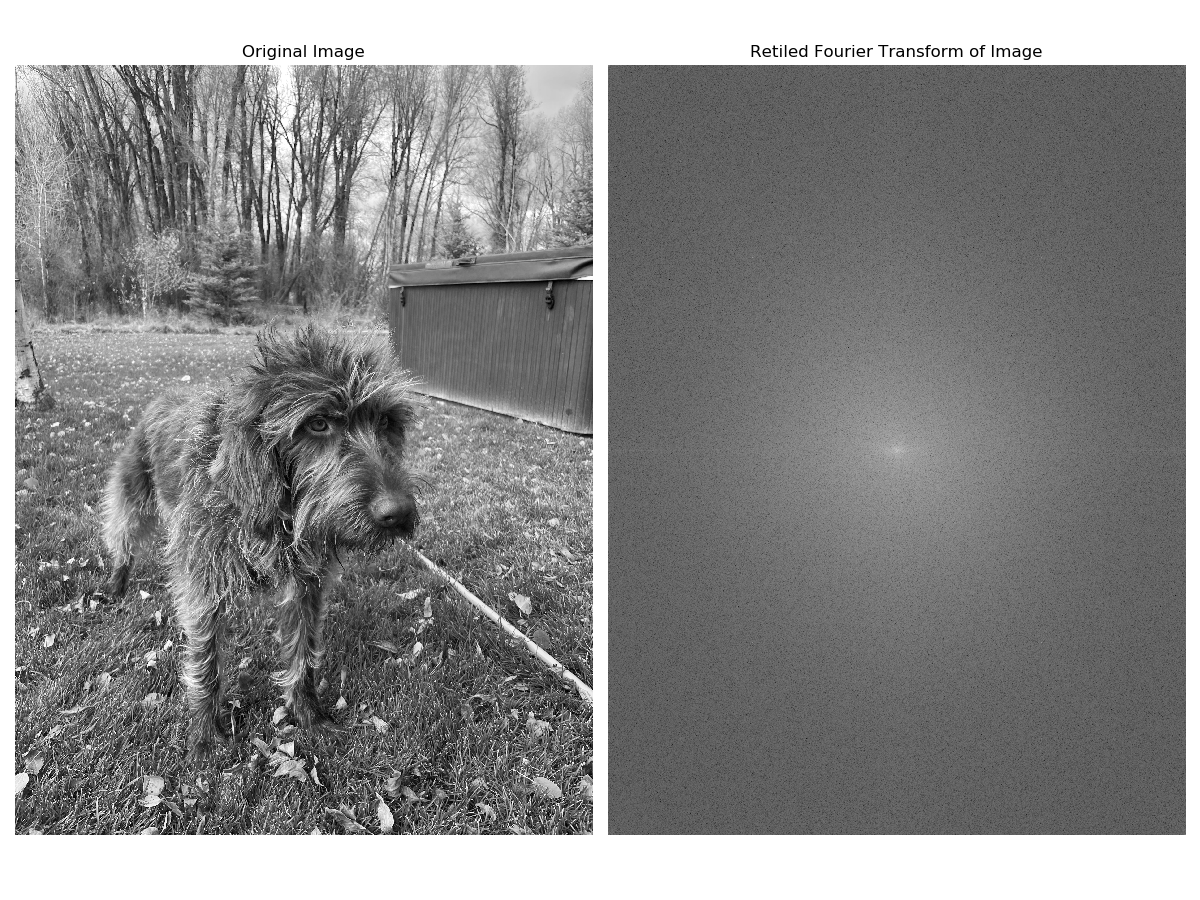
\includegraphics[width=6.5in]{p1_output/img_0_ft_compare.png}
		\caption{Image 0 and its fourier transform}
	\end{figure}
	
%	%-------------------------------------------------------------------------------------------
%	% image 1
%	\begin{figure}[H]
%		\centering
%		\includegraphics[width=6.5in]{p1_output_keep/img_1_t_nl1.png}
%		\caption{Image 1, Noise level = 1}
%	\end{figure}
%	
%	%-------------------------------------------------------------------------------------------
%	% image 2
%	\begin{figure}[H]
%		\centering
%		\includegraphics[width=6.5in]{p1_output_keep/img_2_t_nl1.png}
%		\caption{Image 2, Noise level = 1}
%	\end{figure}
%	
%	
%	%-------------------------------------------------------------------------------------------
%	% image 3
%	\begin{figure}[H]
%		\centering
%		\includegraphics[width=6.5in]{p1_output_keep/img_3_t_nl1.png}
%		\caption{Image 3, Noise level = 1}
%	\end{figure}
%	
%	\newpage
%	
	\textbf{Low Pass Filtering in the Fourier Domain}
	Typically we think of low pass filtering in the spatial domain as convolution of the image with some function. From the properties of the fourier transform we know that convolution in the spatial domain is the same as multiplication in the fourier domain. This means that we can multiply the fourier transform of the image with the fourier transform of our filtering function, and then take the inverse  fourier transform of that product to achieve the same result as convolution in the spatial domain. 
	
	I implemented this in two ways. First, I created a 2D rect$(u,v)$ function in the fourier domain (sinc$(x,y)$). This is shown below:
	
	\begin{figure}[H]
		\centering
		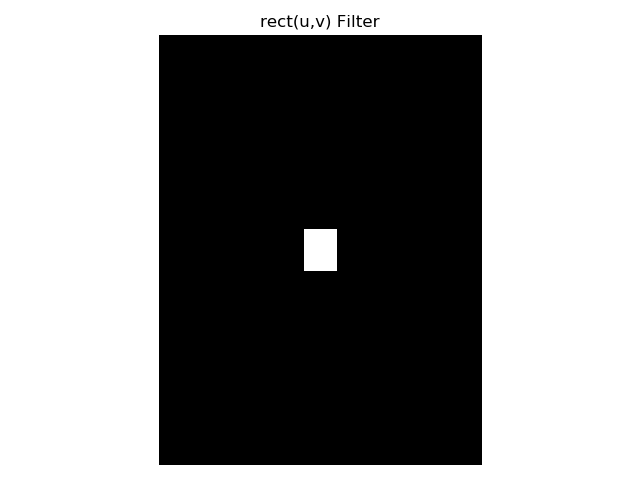
\includegraphics[width=4in]{p1_output/rect_filter.png}
		\caption{rect$(u,v)$ filter in the Fourier Domain}
	\end{figure}
	
	
	I element-wise multiplied each pixel in the filter with each pixel in the image. We know that although this is a mathematically ``ideal" function, in practice it produces artifacts that we are not interested in, like ringing. 
	
	% image 1
	\begin{figure}[H]
		\centering
		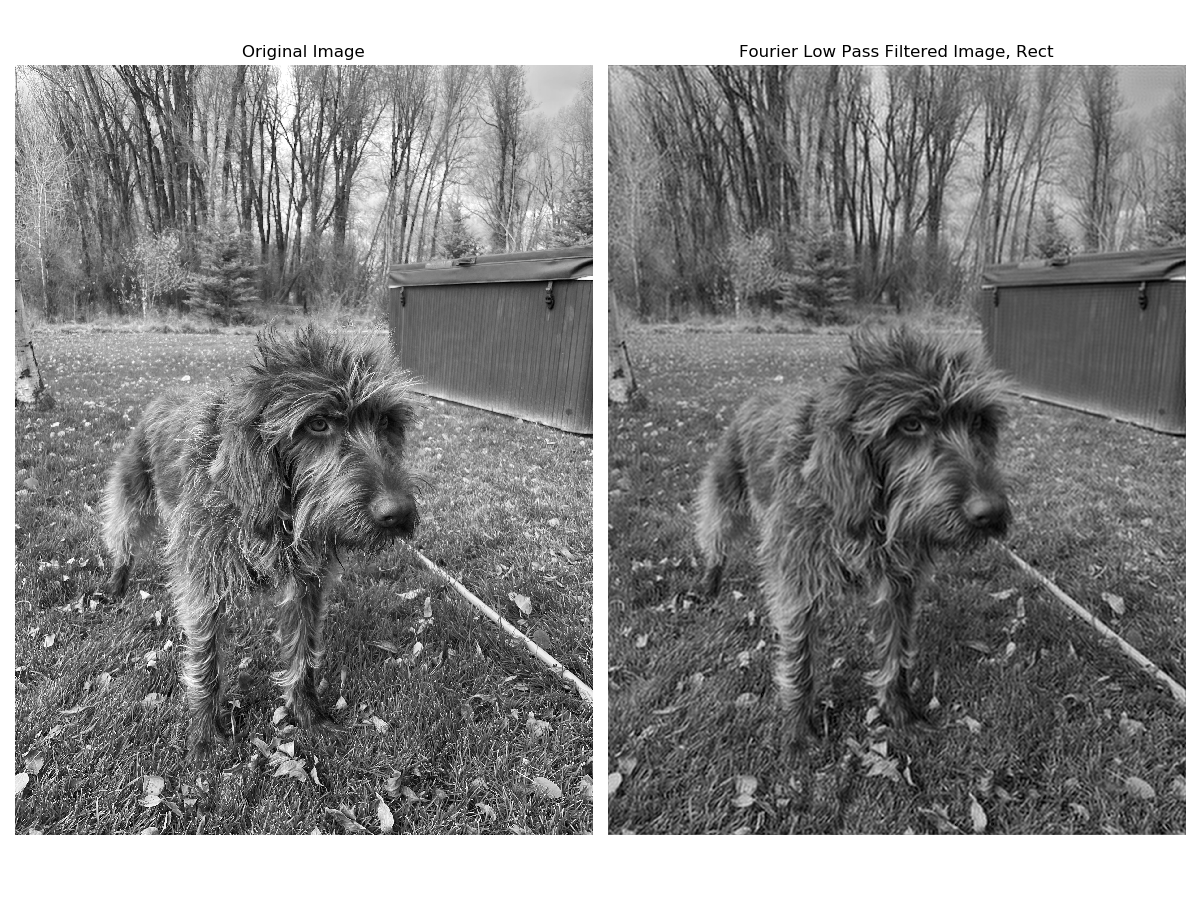
\includegraphics[width=6.5in]{p1_output/img_0_f_rect.png}
		\caption{Original image and fourier-domain rect$(u,v)$ filtered image. Note that this is the same as convolution with a sinc$(x,y)$ function in the spatial domain. This filter appears to darken the image as well}
	\end{figure}
	
	
	Next, I created a 2D Gaussian distribution function in the fourier domain. We know that $\mathcal{F} \{\text{exp}(-\pi u^2)\} = \text{exp}(-\pi x^2)$, i.e. the fourier transform of a gaussian is a gaussian, so it was not necessary that I create this filter in the fourier domain. To make the filter, I multiplied a gaussian in $x$ with a gaussian in $y$:
	%---------------------------------------------------------------------------------
	% gaussian
	\begin{figure}[H]
		\centering
		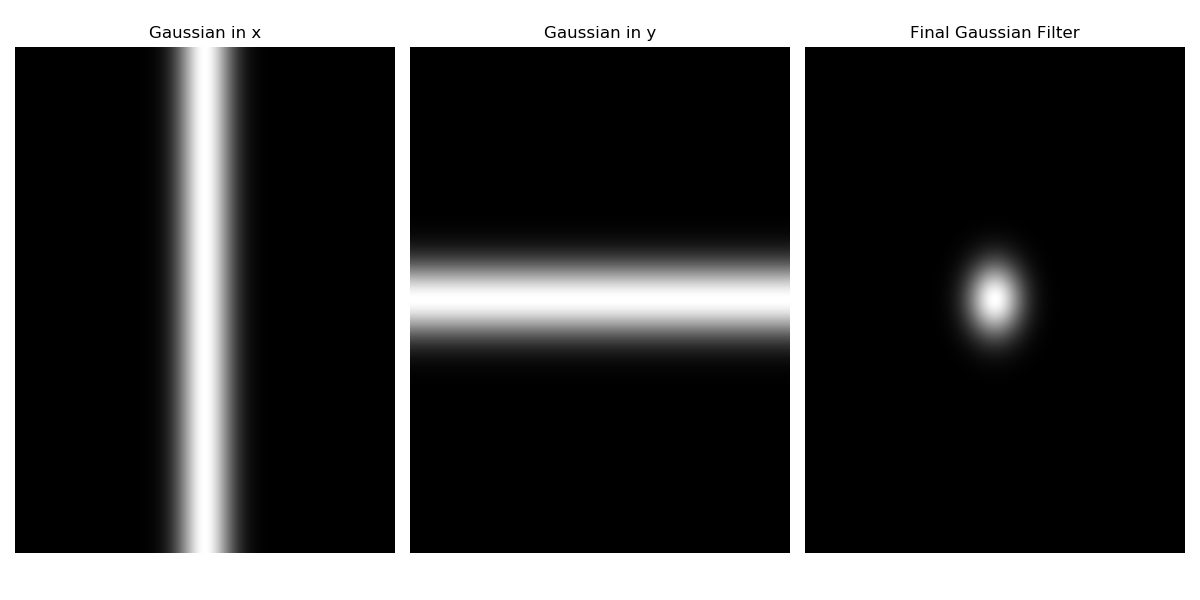
\includegraphics[width=6in]{p1_output/gaussian_filter.png}
		\label{enumeratred_mse}
	\end{figure}

The results of this filter are shown below:
	
	\begin{figure}[H]
		\centering
		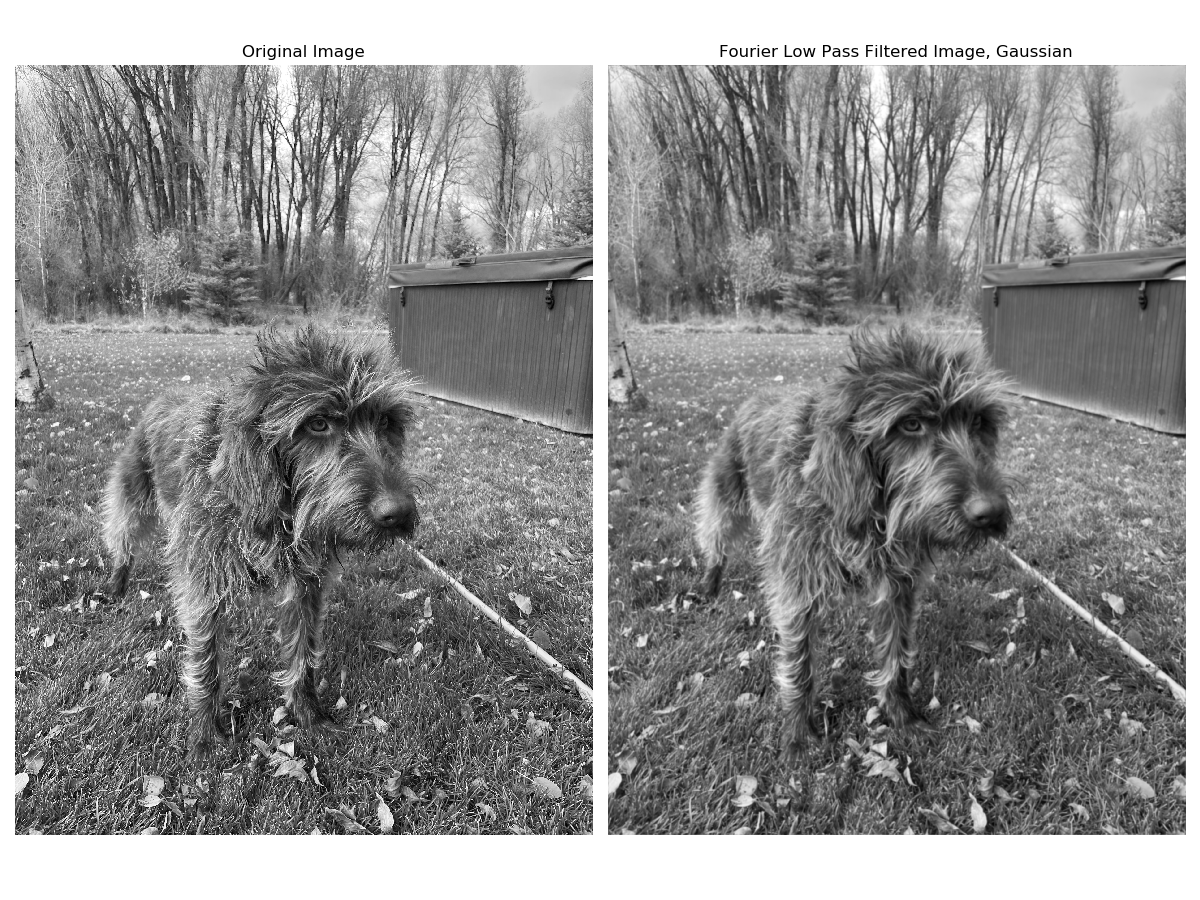
\includegraphics[width=6.5in]{p1_output/img_0_f_gaussian.png}
		\caption{Original image and fourier-domian, gaussian low pass filtered image. Notice the slight blurring in the filtered image.}
	\end{figure}
%	%---------------------------------------------------------------------------------
%	
%	\begin{figure}[H]
%		\centering
%		\includegraphics[width=6.5in]{p1_output_keep/linear_filter_1_sp_3_nl2.png}
%		\caption{Noise level = 2, kernel edge size = 3, Salt and Pepper Noise. From middle-left to bottom right, the MSE of each image is 0.0065, 0.0137, 0.0074, 0.0105, 0.0125 respectively.}
%	\end{figure}
%	%---------------------------------------------------------------------------------
%	% image 2
%	\begin{figure}[H]
%		\centering
%		\includegraphics[width=6.5in]{p1_output_keep/linear_filter_2_g_3_nl2.png}
%		\caption{Noise level = 2, kernel edge size = 3, Gaussian Noise. From middle-left to bottom right, the MSE of each image is 0.0121, 0.0290, 0.0133, 0.0207, 0.0220 respectively.}
%	\end{figure}
%	
%	\begin{figure}[H]
%		\centering
%		\includegraphics[width=6.5in]{p1_output_keep/linear_filter_2_sp_9_nl3.png}
%		\caption{Noise level = 3, kernel edge size = 9, Salt and Pepper Noise. From middle-left to bottom right, the MSE of each image is 0.0142, 0.0282, 0.2307, 0.0129, 0.0360 respectively.}
%	\end{figure}
%	%---------------------------------------------------------------------------------
%	% image 3
%	\begin{figure}[H]
%		\centering
%		\includegraphics[width=6.5in]{p1_output_keep/linear_filter_3_g_9_nl1.png}
%		\caption{Noise level = 1, kernel edge size = 9, Gaussian Noise. From middle-left to bottom right, the MSE of each image is 0.0144, 0.0162, 0.1665, 0.0096, 0.0339 respectively.}
%	\end{figure}
%	
%	\begin{figure}[H]
%		\centering
%		\includegraphics[width=6.5in]{p1_output_keep/linear_filter_3_sp_5_nl2.png}
%		\caption{Noise level = 2, kernel edge size = 5, Salt and Pepper Noise. From middle-left to bottom right, the MSE of each image is 0.0080, 0.0135, 0.0672, 0.0124, 0.0210 respectively.}
%	\end{figure}
%	
%	\textbf{Discussion}
%	As I mentioned above, in every case it appears to me that the averaging filter and the edge weighted filter were the best performing in terms of their ability to reconstruct the image to my subjective liking. However, a study of the MSE only sometimes corroborates this. In general, I found that a larger kernel size resulted in a blurrier image, so although it may have gotten rid of some noise, it went beyond this and altered the structure of the image in a different way. A study of the MSE confirms this as well: for image 0 with Gaussian noise level 1, the MSE for the averaging filter with a kernel edge size of 3 was 0.0091, while for the same noise level and filter but with a kernel edge size of 9, the MSE was 0.0109, some 16\% higher. 
%	
%	Image 1 served as a good test of the filter's ability to preserve predictable details that are not strictly vertical or horizontal. The original image shows many concentric circles of thin wire, and some well-performing filters were able to recover this. In the example shown with a kernel size of 9, it is easy to see the ``blurring" effect I described above. In the process of removing the noise, the filter makes the image look more like the camera was shaky or out of focus when the picture was taken.
%	
%	Both the averaging and edge weighted filters were able to recover the intricate details of the text in image 3 when the image had salt and pepper noise at level 2 and the filters had kernel edge size = 5. At noise level 3 with a kernel edge size of 9 however, the text was not recoverable. This is to be expected though, as this is the highest noise level and the worst performing kernel size. 
%	
%	\newpage
%	
	\section{Part 2: Phase Correlation}
	Please see \texttt{problem\_2.py} for my implementation of this part. Please note that to run the code you will need \texttt{numba}. 
	
	First, I implemented raw phase correlation with no low pass filtering. This works according to the following equation:
	\[p(x, y)=\mathbb{F}^{-1}\left[\frac{F^{*}(u, v) G(u, v)}{\left|F^{*}(u, v) G(u, v)\right|}\right]\]
	
	%---------------------------------------------------------------------------------
	% image 0 bilateral
	\begin{figure}[H]
		\centering
		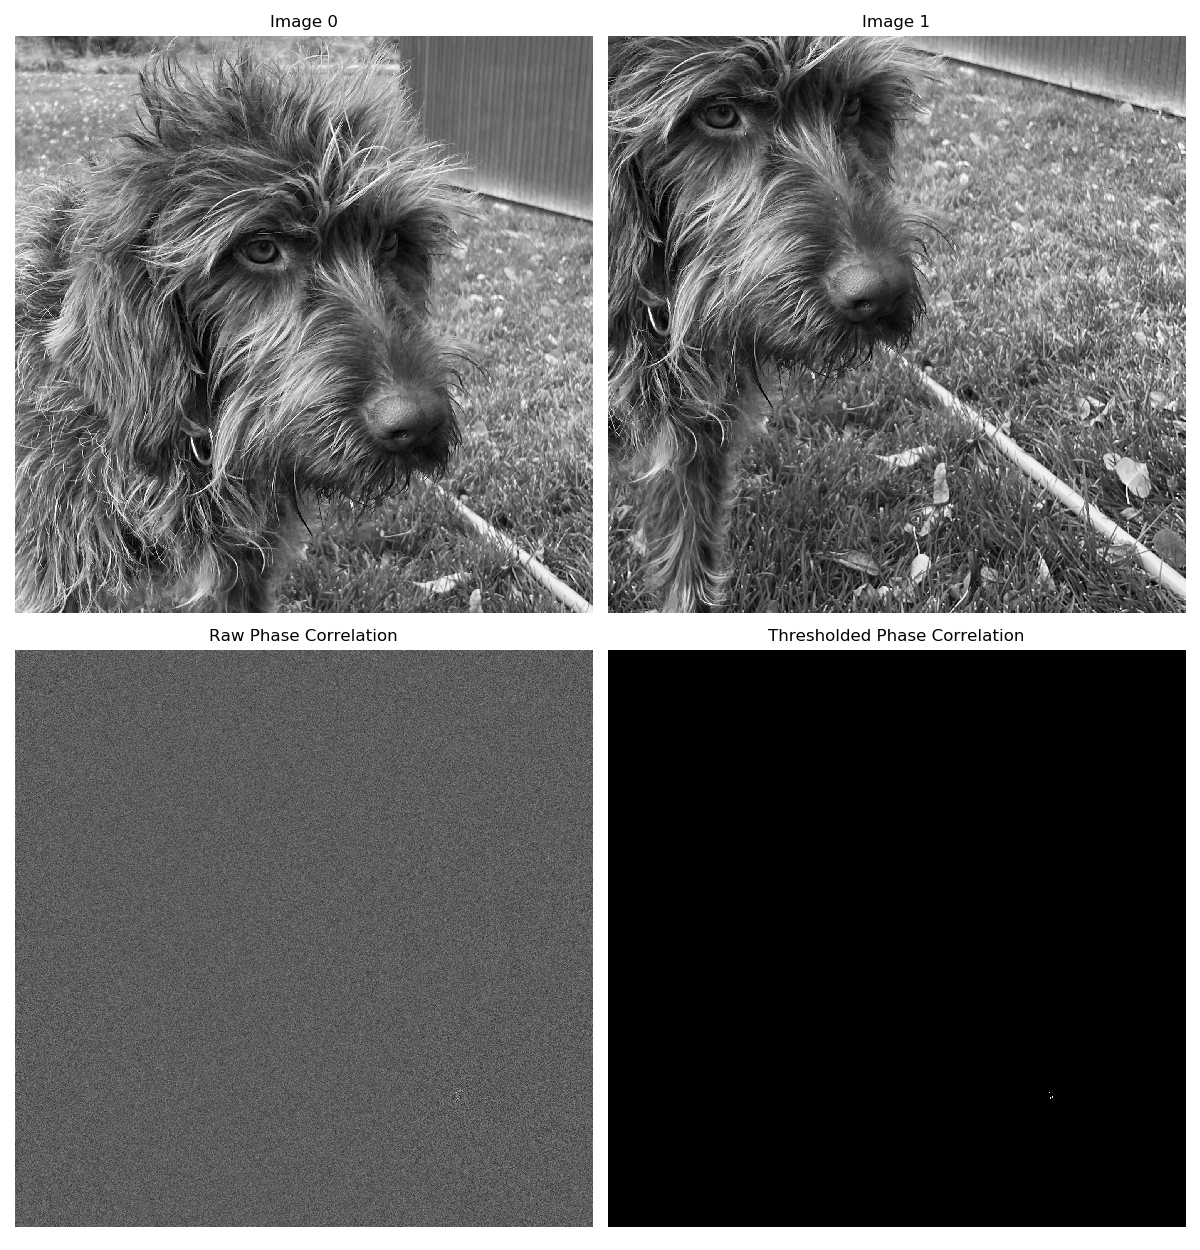
\includegraphics[width=6.5in]{p2_output/phase_correlation_raw.png}
		\caption{Phase correlation of images 0 and 1. The raw correlation data is shown on the left, and a thresholded version is shown on the right. The thresholded version is provided because it is much easier to interpret. See the lower right corner for the pixel of highest intensity.}
	\end{figure}
	
Next, I implemented a low pass filter on the above phase correlation before I took the inverse fourier transform. I used the same gaussian low pass filter from part 1 for this. Curiously, I think these results are worse.
	\begin{figure}[H]
		\centering
		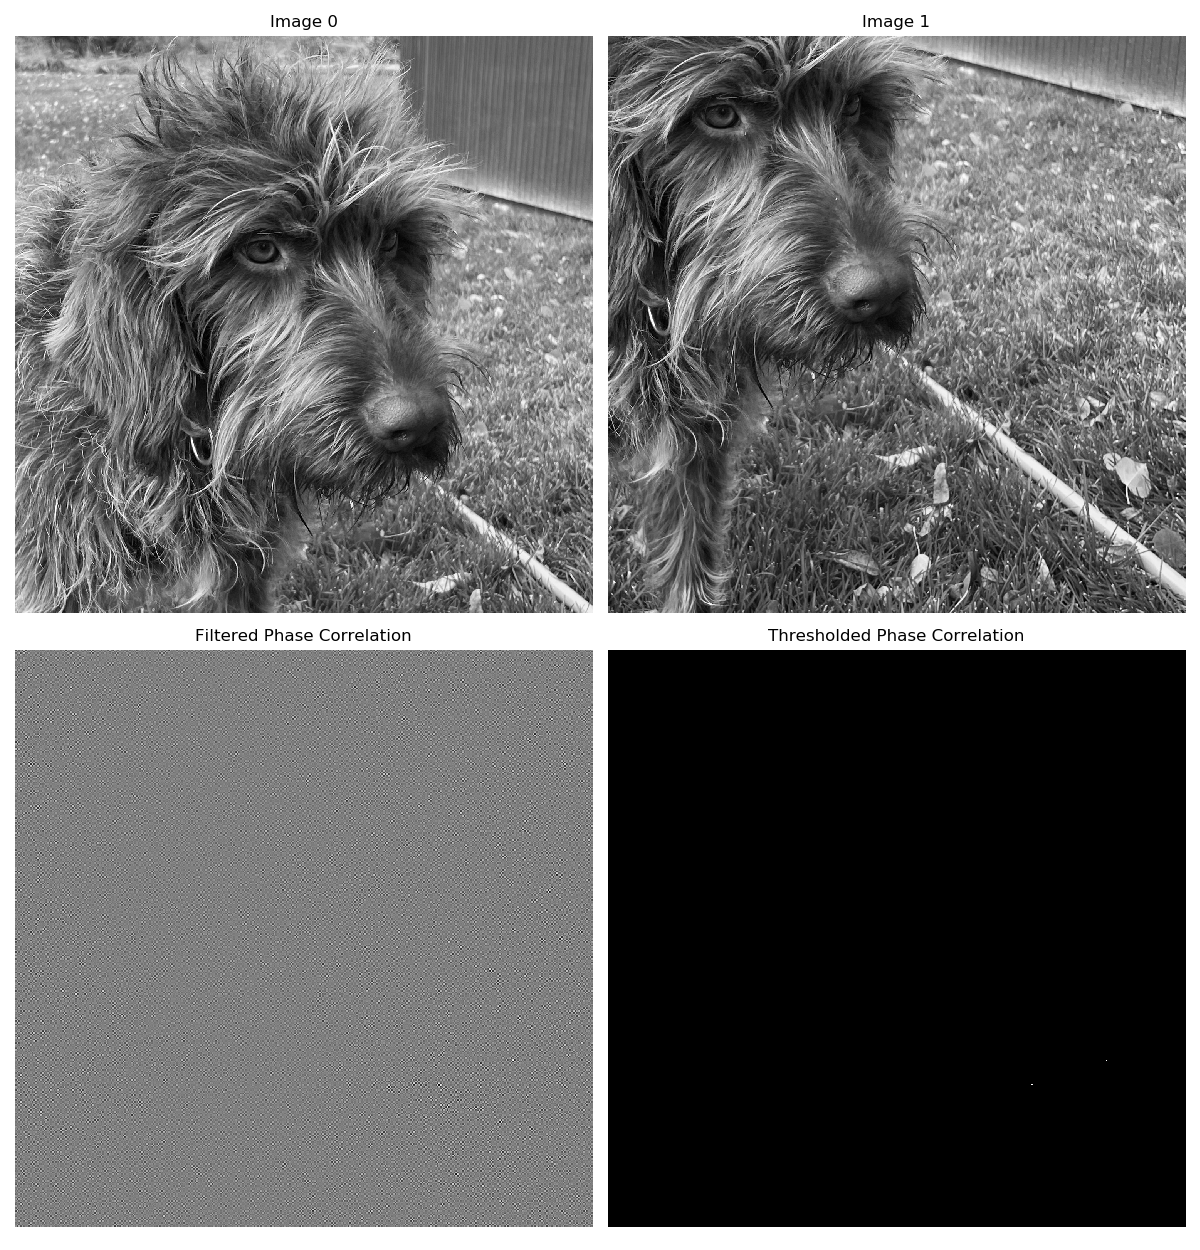
\includegraphics[width=6.5in]{p2_output/phase_correlation_low_pass.png}
		\caption{Phase correlation of images 0 and 1. The low pass filtered correlation data is shown on the left, and a thresholded version is shown on the right. The thresholded version is provided because it is much easier to interpret. it is slightly harder to see, but there is a white pixel at the location of the highest intensity in the lower right corner.}
	\end{figure}

\newpage
\section{Peak Finding}	
\subsection{Algorithm Development - Na\"ive Implementation}
We want to compute the phase correlation of two overlapping images and find the relative location of one with respect to the other so that when we overlay them they line up. Without loss of generality, we will call these images image 1 and image 2.
\begin{figure}[H]
	\centering
	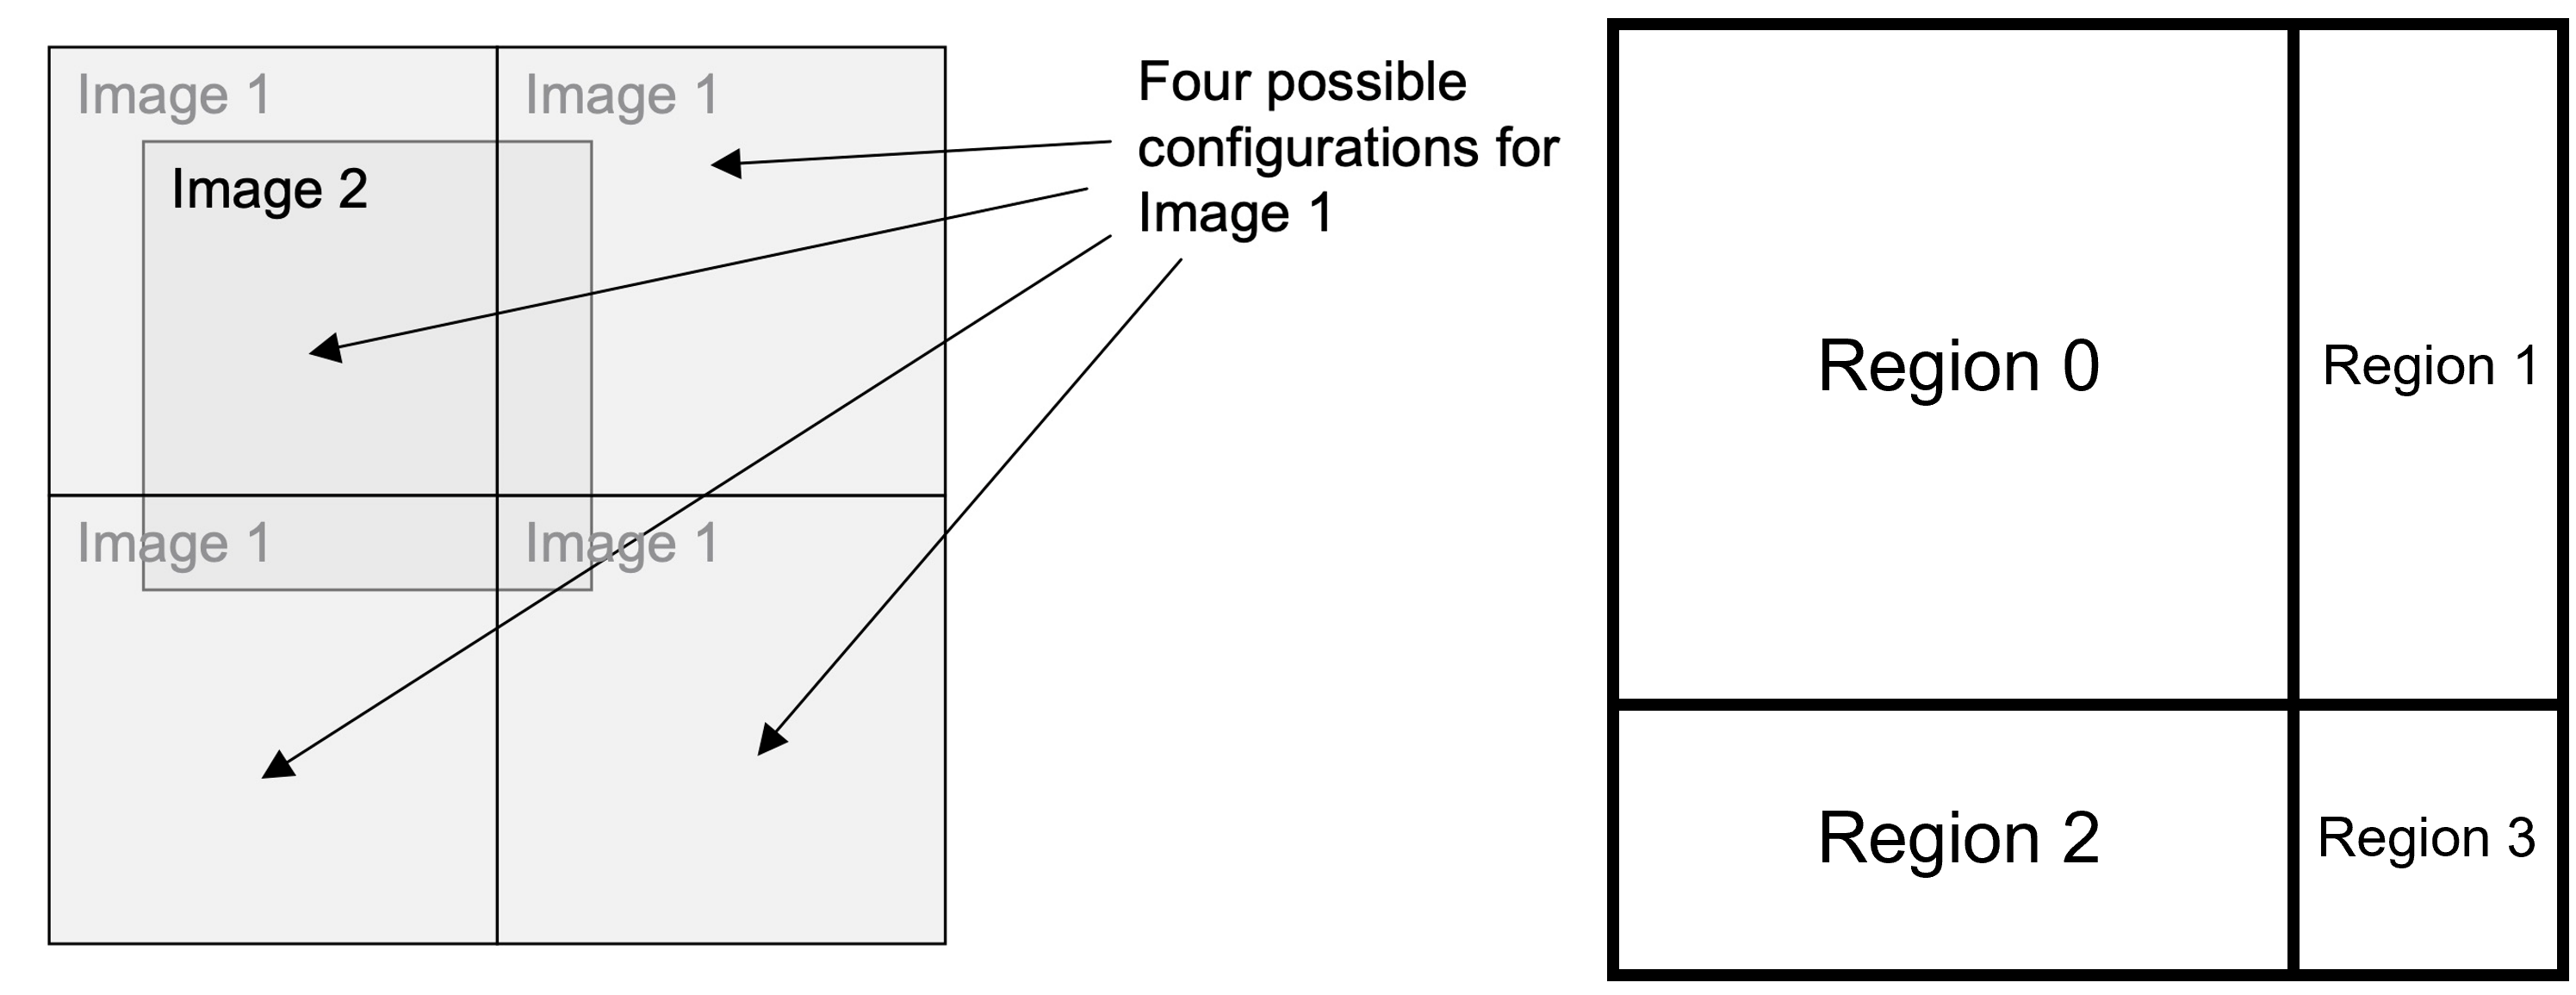
\includegraphics[width=6.75in]{images/region.png}
	\label{regions}
	\caption{Possible locations of image 1 with respect to image 2, and the regions in image 2 defined by these relative locations.}
\end{figure}
Suppose image 1 is an array of $mn$ elements, where $m$ is the number of rows and $n$ is the number of columns. We can only compute the phase correlation of two images if they are of the same size, so it follows that image 2 is an $m$x$n$ array as well. If we compute the phase correlation of images 1 and 2, we have an image where the value of each element is the phase correlation at that location. We can find the indices of the maximal element in the array and call this location $(\lambda _x, \lambda _y)$. Note that in this case, the axis corresponding to the second dimension is defined as positive when we traverse \emph{down} the image, contrary to our intuition from Cartesian axes. We are using python, so as far as the computer is concerned we can say that $(\lambda _x, \lambda _y)\equiv$ \texttt{image2}$[\lambda _y,\lambda _x]$.

\vskip 5pt

\textbf{Region 0:} Consider the placement of image 1 on top of image 2 that defines region 0. In this case, we wish to place the origin of image 1 (the upper left corner) a directed distance of $(-{(n-\lambda _x)},-{(m-\lambda _y)})$ from the origin of image 2. This means that region 0 in image 1 is defined as the rectangle whose vertices are located at $(n-\lambda _x,m-\lambda _y)$, $(n,m-\lambda _y)$, $(n-\lambda_x,m)$, and $(n,m)$. We want to compute the phase correlation of this region with the same region in image 2, whose vertices are located at $(0,0)$, $(\lambda_x,0)$, $(0,\lambda_y)$, and $(\lambda_x,\lambda_y)$. Once we have computed the phase correlation of these two regions, we can record the maximum intensity of the phase correlation.

\vskip 5pt

\textbf{Region 1:} Consider the placement of image 1 on top of image 2 that defines region 1. In this case, we wish to place the origin of image 1 a directed distance of $(\lambda_x,-{(m-\lambda_y)})$ away from the origin of image 2. Thus, the vertices of region 1 in image 1 are given by $(0,m-\lambda_y)$, $(n-\lambda_x,m-\lambda_y)$, $(0,\lambda_y)$, and $(n-\lambda_x,m)$. The vertices of region 1 in image 2 are $(n-\lambda_x,0)$, $(n,0)$, $(n-\lambda_x, \lambda_y)$, and $(n-\lambda_x,m)$. We then compute the phase correlation of these two regions and record the maximum intensity of the phase correlation.

\vskip 5pt

\textbf{Region 2:} Consider the placement of image 1 on top of image 2 that defines region 2. In this case, we wish to place the origin of image 1 a directed distance of $(-(n-\lambda_x),\lambda_y)$ away from the origin of image 2. Thus, the vertices of region 2 in image 1 are given by $(n-\lambda_x,0)$, $(n,0)$, $(n-\lambda_x,m-\lambda_y)$, and $(n,m-\lambda_y)$. The vertices of region 2 in image 2 are $(0,\lambda_y)$, $(\lambda_x,\lambda_y)$, $(0,m)$, and $(\lambda_x,m)$. Once again, we compute the phase correlation of these two regions and record the maximum intensity.

\vskip 5pt

\textbf{Region 3:} Finally, consider the placement of image 1 on top of image 2 that defines region 3. In this case, we wish to place the origin of image 1 a directed distance of $(\lambda_x,\lambda_y)$ away from the origin of image 2. Thus, the vertices of region 3 in image 1 are given by $(0,0)$, $(n-\lambda_x,0)$, $(0,m-\lambda_y)$, and $(n-\lambda_x,m-\lambda_y)$. The vertices of region 3 in image 2 are $(\lambda_x,\lambda_y)$, $(n,\lambda_y)$, $(\lambda_x,m)$, and $(n,m)$. For the last time we compute the phase correlation of these two regions and record the maximum intensity.

Now we have four maximum intensities, one coming from each region. We expect three of them to be meaningless (though not necessarily of the same value or order of magnitude) and one to be the maximal among the four. The region which contributes this intensity dictates the appropriate placement of image 1 on top of image 2. 

Now we must define a canvas on which to place the images so we can visually inspect the results of this approach. We can easily determine the size of the canvas based on our new knowledge of the correct location of image 1 with respect to image 2. If we end up with region 0, the canvas must have $(2n-\lambda_x)$ columns and $(2m-\lambda_y)$ rows. If we end up with region 1, the canvas must have $(n+\lambda_x)$ columns and $(2m-\lambda_y)$ rows. If we end up with region 2, the canvas must have $(2n-\lambda_x)$ columns and $(m+\lambda_y)$ rows. Finally, if we end up with region 3, the canvas must have $(n+\lambda_x)$ columns and $(m+\lambda_y)$ rows. 

\newpage
\subsection{Results - Na\"ive Implementation}
Using the above algorithm I was able to take the following pairs of images:
\begin{figure}[H]
	\centering
	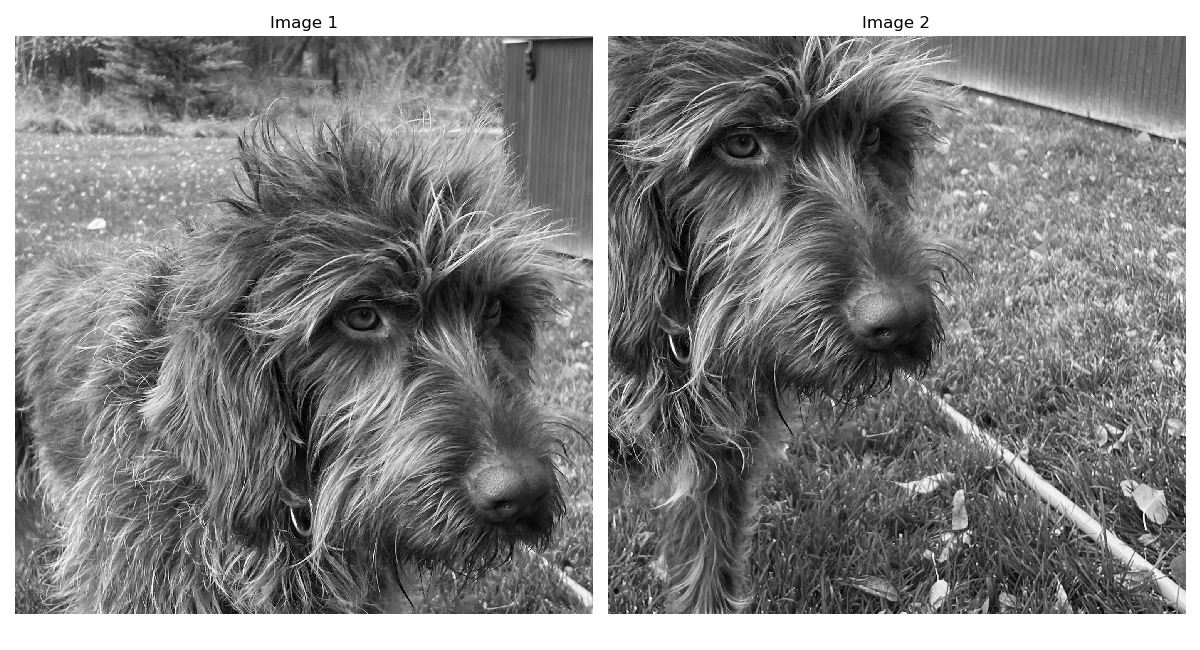
\includegraphics[width=6.5in]{p3_output/img_0_pieces.png}
\end{figure}

\begin{figure}[H]
	\centering
	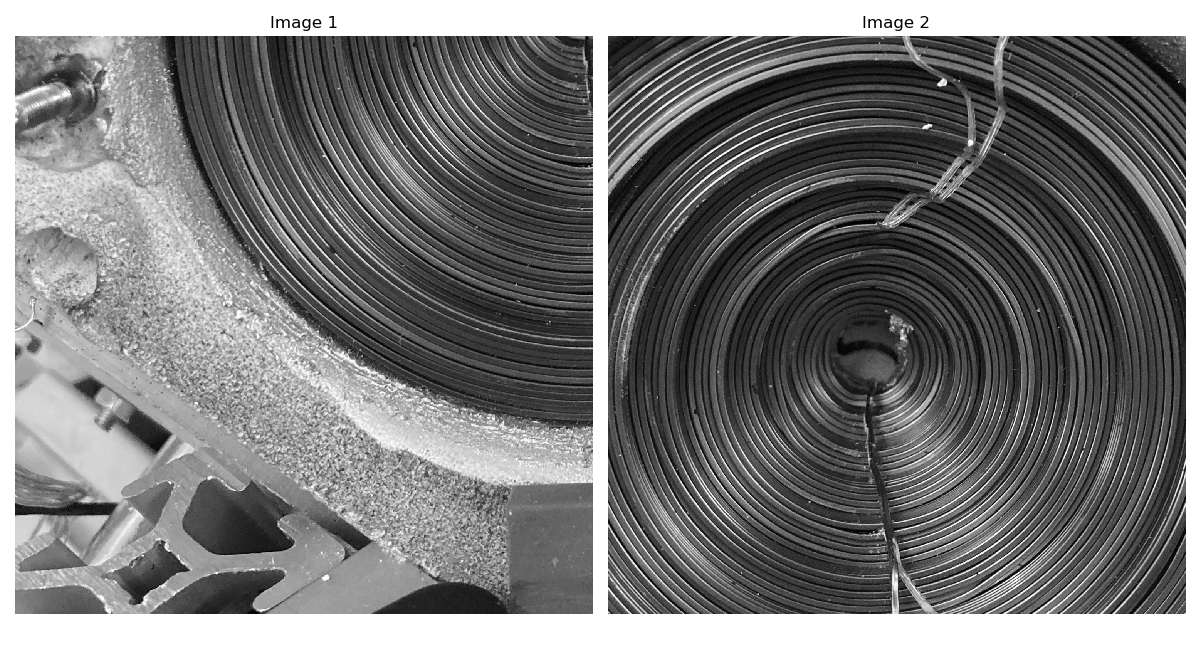
\includegraphics[width=6.5in]{p3_output/img_1_pieces.png}
\end{figure}
And stitch them together into the following mosaics:

\begin{figure}[H]
	\centering
	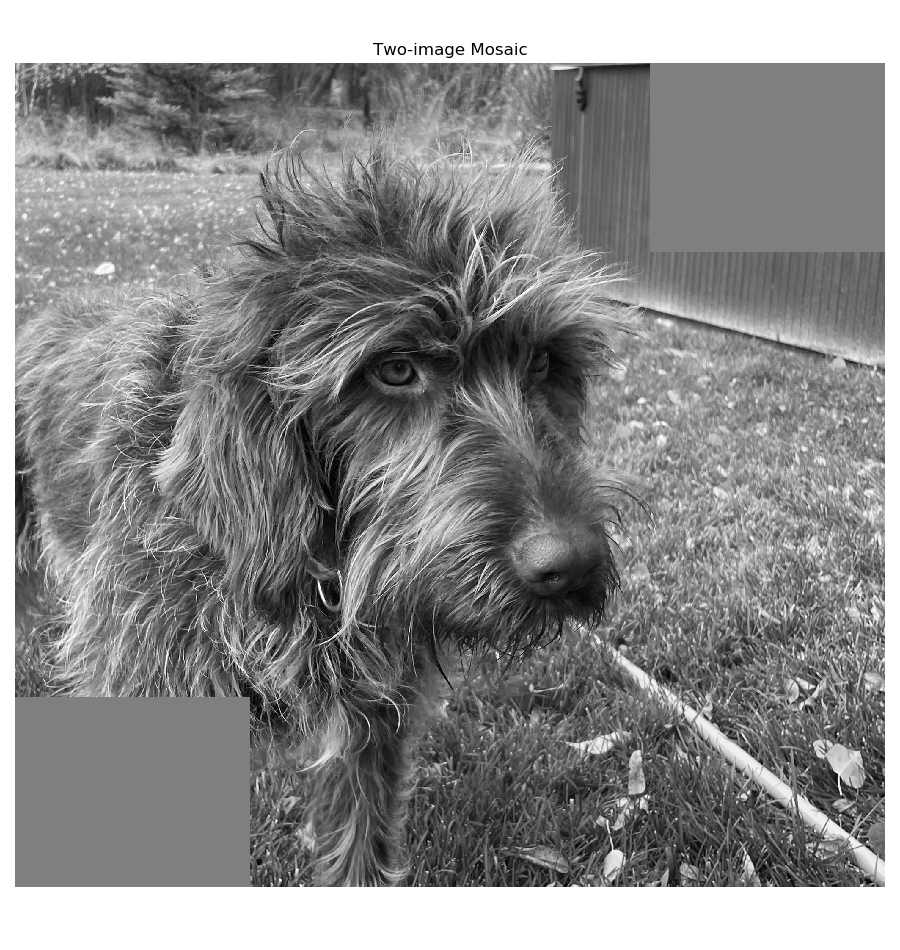
\includegraphics[width=6.5in]{p3_output/img_0_mosaic.png}
\end{figure}

\begin{figure}[H]
	\centering
	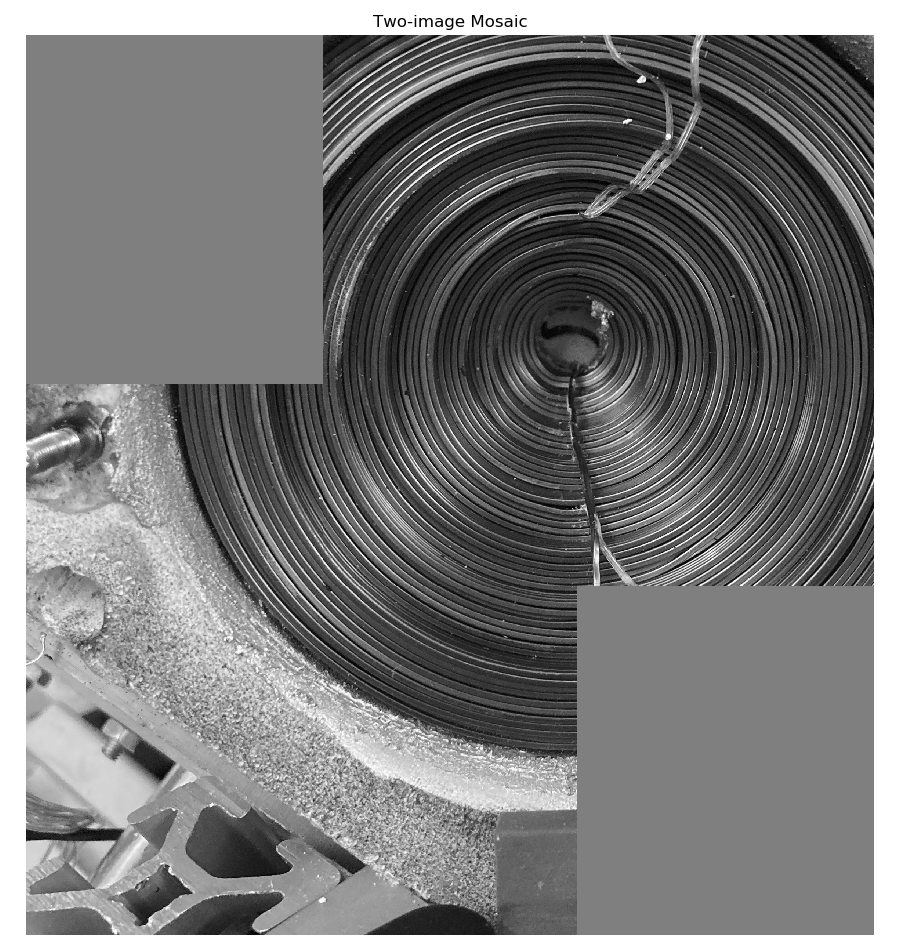
\includegraphics[width=6.5in]{p3_output/img_1_mosaic.png}
\end{figure}
\vskip 5pt
I have called this the ``na\"ive implementation" because I am simply finding the maximum phase correlation and locating purely based on that metric. This has no built in low-pass filtering method (like finding centroids of connected components, or some other clever method) and could be susceptible to unforseen difficulties relating to high frequency noise. However, this is unlikely because we can think of high frequency noise as being related to the number of sharp edges in an image. But, both of these images are composed of many high frequency signals so if this method really were so delicate, these particular images should expose this weakness. However, looking at the results we can see that these reconstructions are nearly perfect, indicating that this is a valid way of constructing mosaics that appears to be immune to high frequency noise.

\end{document}          

